\documentclass[conference]{IEEEtran}
\usepackage{cite}
\usepackage{amsmath,amssymb}
\usepackage{graphicx}
\usepackage{booktabs}
\usepackage{siunitx}
\usepackage{tikz}
\usetikzlibrary{arrows.meta,calc,positioning,shapes.geometric}
\usepackage{hyperref}
\hypersetup{hidelinks}
\sisetup{round-mode=places,round-precision=4}

\title{Conditional Drifting Models for Learned Channel Simulation:\\
Detailed Experimental Draft and Comparison With Diffusion and GAN Baselines}

\author{
\IEEEauthorblockN{Anonymous Submission}
\IEEEauthorblockA{DM\_for\_learning\_channels}
}

\begin{document}
\maketitle

\begin{abstract}
Accurate stochastic channel simulation is central to data-driven communication system design, especially when measured channels are costly to acquire repeatedly or when differentiable learned surrogates are needed inside end-to-end optimization loops.
Recent work has shown that conditional diffusion models are strong channel generators, but their inference cost scales with the number of reverse denoising steps.
This paper studies conditional drifting models as a low-latency alternative and evaluates them against conditional DDPM, conditional DDIM, and conditional GAN baselines.
All models are trained in residual space to approximate the conditional law of \(e = y - x\), where \(x\) denotes the transmitted symbol and \(y\) the channel output.
The benchmark covers AWGN, Rayleigh fading, SSPA nonlinearity, and a simplified optical-fiber proxy channel.
Our drifting implementation is a practical conditional adaptation of the recently proposed drifting-model idea \cite{drifting}, using an attraction--repulsion drift field on generated residual samples.
In the current benchmark, drifting is competitive or best in lower-budget settings and remains strongest on Rayleigh and the optical-fiber proxy at \(T=100\), while DDPM(100) achieves the best sliced Wasserstein distance on AWGN and SSPA.
A separate timing study over 20{,}480 samples shows that one-shot drifting is \(260.8\times\) faster than DDPM(100) on CPU.
These results position drifting as a promising fast alternative to iterative diffusion-based channel generators.
\end{abstract}

\begin{IEEEkeywords}
learned channel models, conditional generative modeling, diffusion models, drifting models, sliced Wasserstein distance, inference latency
\end{IEEEkeywords}

\section{Introduction}
Accurate channel models are a basic requirement for modern communication-system design.
They are especially important in neural and end-to-end learned systems, where the channel appears repeatedly inside training loops, decoder adaptation procedures, and differentiable autoencoder pipelines.
When a clean analytical channel model is unavailable, too restrictive, or poorly matched to measured data, generative channel surrogates become attractive because they can learn the full conditional distribution directly from samples.

This problem is not only about fidelity.
In many learning pipelines, the channel model is evaluated millions of times.
As a result, sample quality, conditioning fidelity, computational cost, and differentiability all matter simultaneously.
The question is therefore not merely whether a generative model can match the channel distribution, but whether it can do so at a cost compatible with large-scale training and deployment workflows.

Recent work on diffusion-based channel modeling has shown that conditional diffusion models can generate high-quality channel samples across standard benchmarks such as AWGN, Rayleigh, and nonlinear amplifier channels \cite{paper2309}.
That line of work is compelling because diffusion models are flexible, robust, and often more stable than earlier adversarial approaches.
However, this improvement comes with a practical systems cost: inference requires an iterative reverse denoising procedure, and the latency scales with the number of diffusion steps.
This tradeoff is manageable when the channel generator is called occasionally, but it becomes more problematic when it is embedded in inner loops of iterative training or repeated Monte Carlo evaluation.

This motivates the study of one-shot conditional generators for learned channel simulation.
Among recently proposed generative paradigms, drifting models \cite{drifting} are particularly interesting because they aim to learn the transport from a simple latent source to the target data distribution directly in the network parameters, rather than unfold that transport as a multi-step sampling trajectory at inference time.
Intuitively, diffusion spends computation at test time by progressively transforming noise into data through a reverse-time chain.
Drifting instead spends computation during training: generated samples are repeatedly nudged toward the data manifold by a drift field, and the neural generator is updated so that future samples move closer to the desired distribution in a single forward pass.
Once trained, sampling is therefore naturally one-shot.

That distinction makes drifting conceptually appealing for channel modeling.
In a communication setting, the generator must be conditional on the transmitted symbol \(x\), and it must capture not just a marginal sample cloud, but the conditional law \(p(y \mid x)\).
The recently proposed drifting framework is still new, and in the context of communication channels there is no widely adopted baseline yet.
This makes it important to document not only benchmark results, but also the concrete conditional adaptation required to make drifting operational in a channel-learning codebase.

The goal of this draft is therefore twofold.
First, we extend the existing diffusion-based channel-learning repository of \cite{paper2309} with a practical conditional drifting baseline, a stronger conditional GAN baseline, and an optical-fiber proxy channel adapted from \texttt{DM\_OptFib}.
Second, we benchmark these models under a common residual-space evaluation protocol using sliced Wasserstein distance (SWD), together with direct timing measurements.
The emphasis of this draft is on generator-level distributional fidelity and computational tradeoffs rather than on downstream symbol-error-rate curves.

The main contributions are summarized as follows.
\begin{itemize}
\item We formulate a conditional drifting generator for channel simulation by modeling residuals \(e = y - x\) and conditioning the generator directly on the transmitted symbol.
\item We provide a practical drifting objective based on attraction and repulsion in residual space, which is straightforward to integrate into an existing PyTorch channel-learning pipeline.
\item We compare conditional DDPM, conditional DDIM, conditional GAN, and conditional drifting models on AWGN, Rayleigh, SSPA, and optical-fiber proxy channels.
\item We quantify the fidelity--latency tradeoff and show that one-shot drifting provides large inference-time savings while remaining competitive in distributional fidelity.
\end{itemize}

\section{Problem Formulation and Model Background}
\subsection{Residual-space conditional channel modeling}
Let \(x \in \mathbb{R}^n\) denote the transmitted channel input and \(y \in \mathbb{R}^n\) the channel output.
Rather than learn \(p(y \mid x)\) directly, we model the residual
\begin{equation}
e = y - x.
\end{equation}
Each generator is trained to approximate the conditional residual law \(p(e \mid x)\), and generated channel outputs are reconstructed as
\begin{equation}
\hat{y} = x + \hat{e}.
\end{equation}
This representation has two practical benefits in the present benchmark.
First, it places additive and non-additive channels on a more comparable footing by centering the learning target around the input symbol.
Second, it makes evaluation more interpretable, because the residual distribution directly expresses what the channel adds, scales, or distorts relative to the transmitted signal.

\subsection{Conditional diffusion baseline}
The diffusion baseline follows the channel-learning setting of \cite{paper2309} and uses the epsilon-prediction DDPM objective \cite{ddpm} with DDIM sampling \cite{ddim} as a deterministic alternative at inference time.
The denoiser is a conditional multilayer perceptron
\begin{equation}
\epsilon_\theta(e_t, t, x),
\end{equation}
where \(e_t\) is a noisy residual at diffusion step \(t\).
In the benchmark implementation, the residual dimension is \(n=2\), the hidden width is \(128\), the first layer receives the concatenated vector \([e_t, x]\), and each hidden layer is modulated by a learned time embedding.
Softplus nonlinearities are used throughout the hidden stack.

Training uses a cosine noise schedule.
Given a clean residual \(e_0\), a random step \(t\), and Gaussian noise \(\epsilon\), the denoiser is optimized by
\begin{equation}
\mathcal{L}_{\text{DDPM}}
=
\mathbb{E}_{e_0, x, t, \epsilon}
\left[
\left\|
\epsilon - \epsilon_\theta(e_t, t, x)
\right\|_2^2
\right].
\end{equation}
At inference time, DDPM uses the full stochastic reverse chain, whereas DDIM follows a deterministic trajectory with the same trained denoiser.
The important structural point for this paper is that both procedures require a sequence of reverse denoising evaluations, so inference cost scales with the chosen trajectory length.

\subsection{What drifting changes conceptually}
Because drifting is still unfamiliar to many readers, it is useful to state its generative viewpoint explicitly.
Following \cite{drifting}, let \(f_\theta\) map a latent variable \(z \sim p_z\) to a sample \(u = f_\theta(z)\), and let
\begin{equation}
q_\theta = (f_\theta)_\# p_z
\end{equation}
denote the pushforward distribution induced by the generator.
The training objective is no longer expressed as a likelihood surrogate or as a denoising score-matching loss.
Instead, the paper introduces a \emph{drifting field} that tells us how samples drawn from the current model distribution should move so that the model distribution approaches the target distribution \(p\).

At a high level, the desired property is an equilibrium condition:
if the model already matches the target distribution, then the drift should vanish.
Using \(V_{p,q}(u)\) to denote the field evaluated at a sample \(u\) under target distribution \(p\) and model distribution \(q\), the fixed-point intuition can be summarized as
\begin{equation}
q = p
\quad \Longrightarrow \quad
V_{p,q}(u) = 0,
\end{equation}
which is the sense in which matched distributions form an equilibrium of the training dynamics \cite{drifting,driftingproj}.

This makes the training logic very different from diffusion.
In diffusion, one learns a denoiser and then performs iterative refinement at inference time.
In drifting, one instead constructs improved targets during training by moving current samples along the field \(V_{p,q}\), and then regresses the generator onto those improved targets.
As a result, the iterative correction happens during optimization rather than at test time.

The paper-level one-step view can be written as follows.
Starting from a generated sample \(u = f_\theta(z)\), define a drifted target
\begin{equation}
\tilde{u}
=
\mathrm{stopgrad}\!\left(
u + \eta V_{p,q_\theta}(u)
\right),
\end{equation}
and optimize the generator by
\begin{equation}
\mathcal{L}_{\text{drift}}
=
\mathbb{E}_{z \sim p_z}
\left[
\left\|
f_\theta(z) - \tilde{u}
\right\|_2^2
\right].
\end{equation}
The stop-gradient is essential here: it makes the drifted sample behave like a fixed target for the current optimization step.
Repeated training steps therefore evolve the pushforward \(q_\theta\) toward the target distribution.
This is also the cleanest way to see why drifting is naturally one-shot at inference:
once the generator has learned to emit samples near equilibrium, sampling only requires drawing \(z\) and evaluating \(f_\theta(z)\), with no reverse-time chain.

Fig.~\ref{fig:toy} gives an actual toy particle simulation in the spirit of the particle-based demonstrations used in \cite{drifting}.
For two fixed channel inputs, we initialize mismatched conditional residual particle clouds and then evolve them under the same attraction--repulsion drift rule used in our channel benchmark.
The figure therefore illustrates real drift dynamics rather than a hand-drawn schematic, while still serving only as a toy analogue of the full learned generator.
To show that the same idea can train an explicit parameterized generator, Fig.~\ref{fig:toymlp} uses a tiny conditional MLP trained with the drifting objective on the same toy target.
For contrast, Fig.~\ref{fig:toydiff} shows an oracle conditional diffusion-style reverse trajectory on the same target, making the difference in sampling path length visually explicit.

\subsection{Conditional drifting baseline}
Our implementation should be viewed as a practical conditional adaptation inspired by \cite{drifting}, rather than as an exhaustive reproduction of every variant in that paper.
To avoid confusion with the communication input symbol \(x\), we use \(u\) above for the generic sample variable in the paper-level formulation and reserve \(x\) below for the transmitted symbol.
In the channel-learning benchmark, the target object is the residual \(e = y - x\), and conditioning enters through the transmitted symbol.
The generator is therefore
\begin{equation}
\hat{e} = g_\theta(x, z),
\qquad
z \sim \mathcal{N}(0, I),
\end{equation}
and is implemented as a two-hidden-layer multilayer perceptron with hidden width \(128\), latent dimension \(16\), and SiLU activations:
\begin{equation}
[x, z]
\rightarrow
\mathrm{Linear}
\rightarrow
\mathrm{SiLU}
\rightarrow
\mathrm{Linear}
\rightarrow
\mathrm{SiLU}
\rightarrow
\mathrm{Linear}.
\end{equation}

The training target is formed from an attraction--repulsion drift field in residual space.
This should be read as our concrete channel-specific instantiation of the generic paper-level field \(V_{p,q}\).
Given generated samples \(G = \{g_i\}\) and positive residual samples \(P = \{p_j\}\), we compute
\begin{equation}
V(g_i)
=
\left(
\sum_j w^{(P)}_{ij} p_j - g_i
\right)
-
\lambda
\left(
\sum_k w^{(G)}_{ik} g_k - g_i
\right),
\end{equation}
where \(w^{(P)}\) and \(w^{(G)}\) are row-normalized RBF kernel weights.
The first term attracts each generated sample toward a local barycenter of true residual samples, and the second term repels it from nearby generated samples to reduce collapse.
This yields a detached target
\begin{equation}
\tilde{g}_i
=
\mathrm{stopgrad}\!\left(g_i + \eta V(g_i)\right),
\end{equation}
and the generator is optimized by
\begin{equation}
\mathcal{L}_{\text{drift}}
=
\frac{1}{N}
\sum_i
\left\|
g_i - \tilde{g}_i
\right\|_2^2.
\end{equation}
In other words, the generic update \(u \mapsto u + \eta V_{p,q}(u)\) from the drifting formulation is realized here with a kernel-based residual drift field estimated directly from minibatches of true and generated residual samples.
In the corrected benchmark, the drift scale is \(\eta=1.0\), the repulsive weight is \(\lambda=1.0\), the minimum kernel bandwidth is \(0.2\), and the maximum drift norm is \(2.0\).
These settings were chosen because they produced stable residual distributions and materially improved the early AWGN drifting baseline.

The crucial operational consequence is straightforward:
once training is complete, a channel residual sample is obtained by a single evaluation of \(g_\theta(x,z)\).
There is no reverse chain, no ODE solver, and no per-sample iterative schedule at inference.

\subsection{Conditional GAN baseline}
To complement the diffusion and drifting baselines, we also include a conditional adversarial generator adapted from the \texttt{DM\_OptFib} code path.
The generator receives the concatenated input \([x, z]\), where \(z \sim \mathcal{N}(0,I)\), and predicts the full channel output \(\hat{y}\).
Architecturally, it uses an input linear layer, two batch-normalized hidden blocks, a central hidden layer, two additional batch-normalized hidden blocks, and a residual skip from the condition input \(x\) to the output.
The discriminator receives \([y, x]\), processes it with a residual-style multilayer perceptron, concatenates the original input back into the hidden state, and outputs a scalar realism score.

Two adversarial objectives are implemented in the benchmark code: WGAN-GP and a stronger feature-aligned mode denoted \texttt{GAN\_FA}.
The final benchmark uses \texttt{GAN\_FA}, since it was substantially more stable than the plain WGAN-GP baseline in this channel-learning setting.
In \texttt{GAN\_FA}, the discriminator uses BCE-with-logits with label smoothing, while the generator combines an adversarial term with an \(L_1\) reconstruction penalty:
\begin{equation}
\mathcal{L}_{G}
=
\mathcal{L}_{\text{adv}}
+
\alpha
\mathbb{E}\left[\|\hat{y} - y\|_1\right],
\end{equation}
with \(\alpha = 1.0\).
Generator updates are delayed relative to discriminator steps, and the default hidden width is \(128\).

\begin{figure*}[t]
\centering
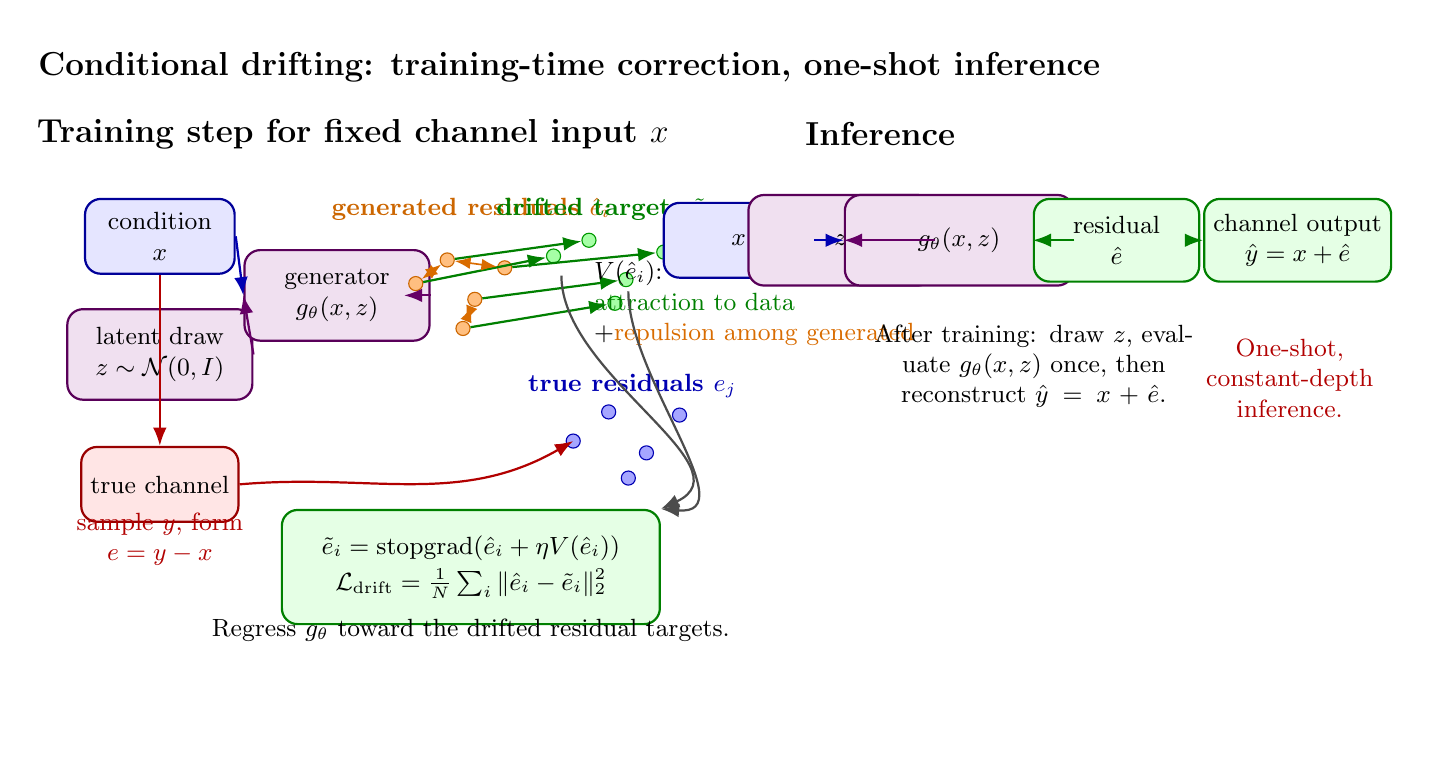
\begin{tikzpicture}[
    >=Latex,
    font=\small,
    boxblue/.style={draw=blue!60!black, thick, rounded corners=2mm, fill=blue!10, minimum width=1.9cm, minimum height=0.95cm, align=center},
    boxviolet/.style={draw=violet!70!black, thick, rounded corners=2mm, fill=violet!12, minimum width=2.35cm, minimum height=1.15cm, align=center},
    boxred/.style={draw=red!60!black, thick, rounded corners=2mm, fill=red!10, minimum width=1.95cm, minimum height=0.95cm, align=center},
    boxgreen/.style={draw=green!50!black, thick, rounded corners=2mm, fill=green!10, minimum width=2.55cm, minimum height=1.05cm, align=center},
    title/.style={font=\bfseries\large},
    note/.style={align=center, font=\small},
    flow/.style={->, thick, draw=black!70},
    attr/.style={->, thick, draw=green!50!black},
    repel/.style={<->, semithick, draw=orange!85!black},
    truedot/.style={circle, draw=blue!70!black, fill=blue!35, inner sep=1.8pt},
    gendot/.style={circle, draw=orange!80!black, fill=orange!50, inner sep=1.8pt},
    targetdot/.style={circle, draw=green!60!black, fill=green!35, inner sep=1.8pt}
]
\fill[white] (-7.5,-4.4) rectangle (9.7,4.5);

% Panel titles
\node[title] at (-1.0,4.0) {Conditional drifting: training-time correction, one-shot inference};
\node[title] at (-3.75,3.15) {Training step for fixed channel input $x$};
\node[title] at (2.95,3.15) {Inference};

% Left panel: inputs and generator
\node[boxblue] (condx) at (-6.2,1.85) {condition\\$x$};
\node[boxviolet] (latent) at (-6.2,0.35) {latent draw\\$z \sim \mathcal{N}(0,I)$};
\node[boxviolet] (gen) at (-3.95,1.1) {generator\\$g_\theta(x,z)$};
\draw[flow, blue!70!black] (condx.east) -- (gen.west);
\draw[flow, violet!80!black] (latent.east) -- (gen.west);

% True channel
\node[boxred] (truech) at (-6.2,-1.3) {true channel};
\draw[flow, red!70!black] (condx.south) -- (truech.north);
\node[note, red!70!black] at (-6.2,-2.0) {sample $y$, form\\$e=y-x$};

% Generated residual cloud
\node[note, orange!80!black] at (-2.25,2.2) {\textbf{generated residuals $\hat e_i$}};
\node[gendot] (g1) at (-2.95,1.25) {};
\node[gendot] (g2) at (-2.55,1.55) {};
\node[gendot] (g3) at (-2.2,1.05) {};
\node[gendot] (g4) at (-1.82,1.45) {};
\node[gendot] (g5) at (-2.35,0.68) {};
\draw[flow, violet!80!black] (gen.east) -- (-3.1,1.1);

% True residual cloud
\node[note, blue!70!black] at (-0.2,-0.05) {\textbf{true residuals $e_j$}};
\node[truedot] (p1) at (-0.95,-0.75) {};
\node[truedot] (p2) at (-0.5,-0.38) {};
\node[truedot] (p3) at (-0.02,-0.9) {};
\node[truedot] (p4) at (0.4,-0.42) {};
\node[truedot] (p5) at (-0.25,-1.22) {};
\draw[flow, red!70!black] (truech.east) to[out=5,in=210] (-0.95,-0.75);

% Drifted targets
\node[note, green!50!black] at (-0.55,2.2) {\textbf{drifted targets $\tilde e_i$}};
\node[targetdot] (t1) at (-1.2,1.6) {};
\node[targetdot] (t2) at (-0.75,1.8) {};
\node[targetdot] (t3) at (-0.28,1.3) {};
\node[targetdot] (t4) at (0.2,1.65) {};
\node[targetdot] (t5) at (-0.42,1.0) {};

% Attraction arrows
\draw[attr] (g1) -- (t1);
\draw[attr] (g2) -- (t2);
\draw[attr] (g3) -- (t3);
\draw[attr] (g4) -- (t4);
\draw[attr] (g5) -- (t5);

% Repulsion arrows
\draw[repel] (g1) -- (g2);
\draw[repel] (g2) -- (g4);
\draw[repel] (g3) -- (g5);

\node[note, align=left] at (1.35,1.0) {$V(\hat e_i)$:\\\textcolor{green!50!black}{attraction to data}\\+\textcolor{orange!85!black}{repulsion among generated}};

% Loss box
\node[boxgreen, minimum width=4.8cm, minimum height=1.45cm] (loss) at (-2.25,-2.35) {$\tilde e_i=\mathrm{stopgrad}\!\left(\hat e_i+\eta V(\hat e_i)\right)$\\[2pt]
$\mathcal{L}_{\mathrm{drift}}=\frac{1}{N}\sum_i \|\hat e_i-\tilde e_i\|_2^2$};
\draw[flow] (-1.1,1.35) to[out=-90,in=25] (loss.north east);
\draw[flow] (-0.25,1.15) to[out=-90,in=-5] (loss.north east);
\node[note] at (-2.25,-3.15) {Regress $g_\theta$ toward the drifted residual targets.};

% Right panel inference
\node[boxblue] (cond2) at (1.15,1.8) {$x$};
\node[boxviolet] (latent2) at (2.45,1.8) {$z$};
\node[boxviolet, minimum width=2.9cm, minimum height=1.15cm] (gen2) at (3.95,1.8) {$g_\theta(x,z)$};
\node[boxgreen, minimum width=2.1cm] (ehat) at (5.95,1.8) {residual\\$\hat e$};
\node[boxgreen, minimum width=2.35cm] (yhat) at (8.25,1.8) {channel output\\$\hat y=x+\hat e$};
\draw[flow, blue!70!black] (cond2.east) -- (gen2.west);
\draw[flow, violet!80!black] (latent2.east) -- (gen2.west);
\draw[flow, green!50!black] (gen2.east) -- (ehat.west);
\draw[flow, green!50!black] (ehat.east) -- (yhat.west);
\node[note, text width=4.6cm] at (4.9,0.2) {After training: draw $z$, evaluate $g_\theta(x,z)$ once, then reconstruct $\hat y=x+\hat e$.};
\node[note, text width=2.8cm, red!70!black] at (8.15,0.05) {One-shot,\\constant-depth inference.};

\end{tikzpicture}
\caption{Illustration of conditional drifting for channel residual modeling. Left: for a fixed transmitted symbol \(x\), the generator produces residual samples \(\hat e_i\), which are moved toward the true residual cloud through a drift field that combines attraction to data and repulsion among generated samples. The network is then regressed toward the drifted targets. Right: after training, inference is one-shot: draw \(z\), evaluate \(g_\theta(x,z)\), and reconstruct the channel output as \(\hat y=x+\hat e\).}
\label{fig:schematic}
\end{figure*}

\begin{figure*}[t]
\centering
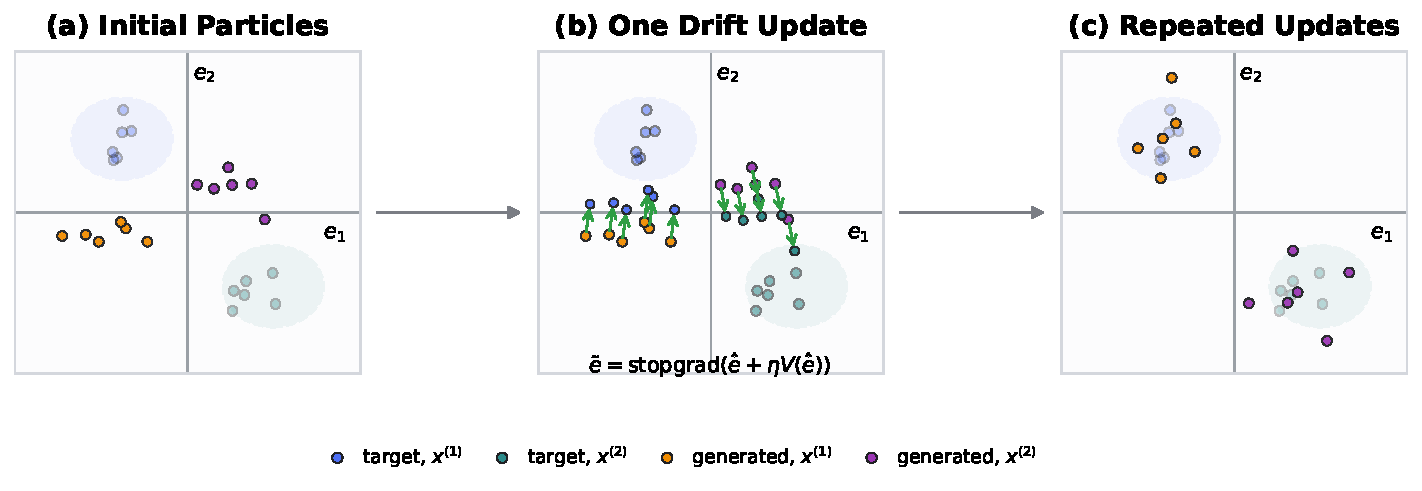
\includegraphics[width=0.95\textwidth]{figures/drifting_conditional_toy_figure_mpl.pdf}
\caption{Toy conditional particle simulation in residual space. Two different channel inputs induce two different target residual distributions. Starting from mismatched generated particle clouds, the middle panel applies one attraction--repulsion drift update of the form \(\tilde e=\mathrm{stopgrad}(\hat e+\eta V(\hat e))\), and the last panel shows the particle clouds after repeated updates. This figure is an actual toy simulation of the drift field, not a hand-drawn schematic.}
\label{fig:toy}
\end{figure*}

\begin{figure*}[t]
\centering
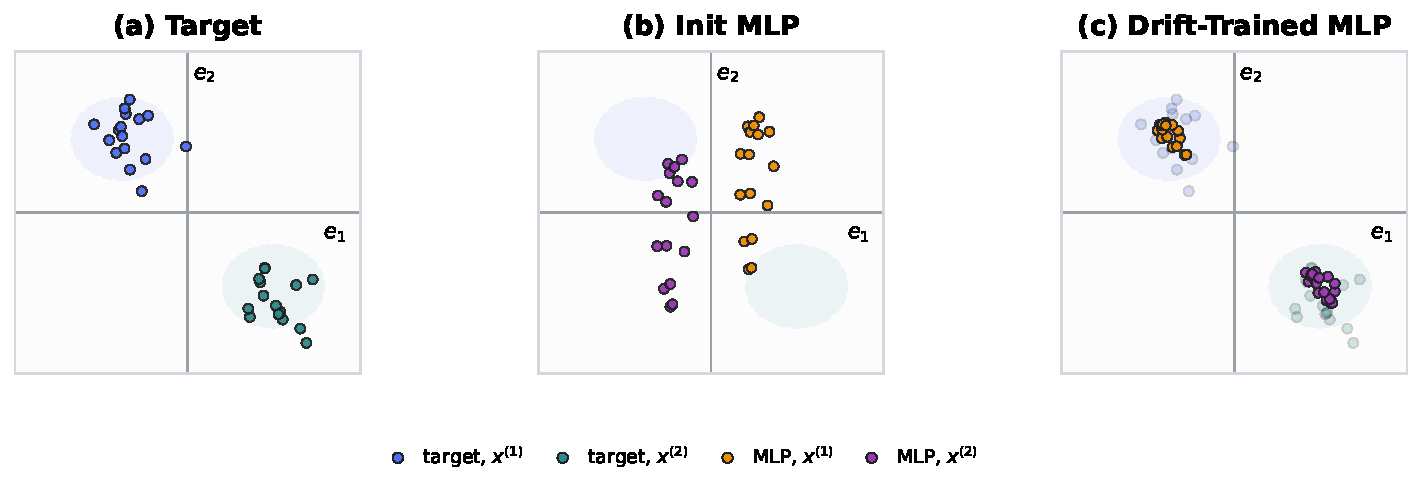
\includegraphics[width=0.95\textwidth]{figures/drifting_tiny_mlp_demo_mpl.pdf}
\caption{Toy conditional MLP trained with the drifting objective. The left panel shows target conditional residual samples. The middle panel shows samples from a randomly initialized tiny conditional MLP \(g_\theta(x,z)\). The right panel shows the same MLP after training with the drift objective, where the generated samples move close to the correct condition-dependent residual clouds.}
\label{fig:toymlp}
\end{figure*}

\begin{figure*}[t]
\centering
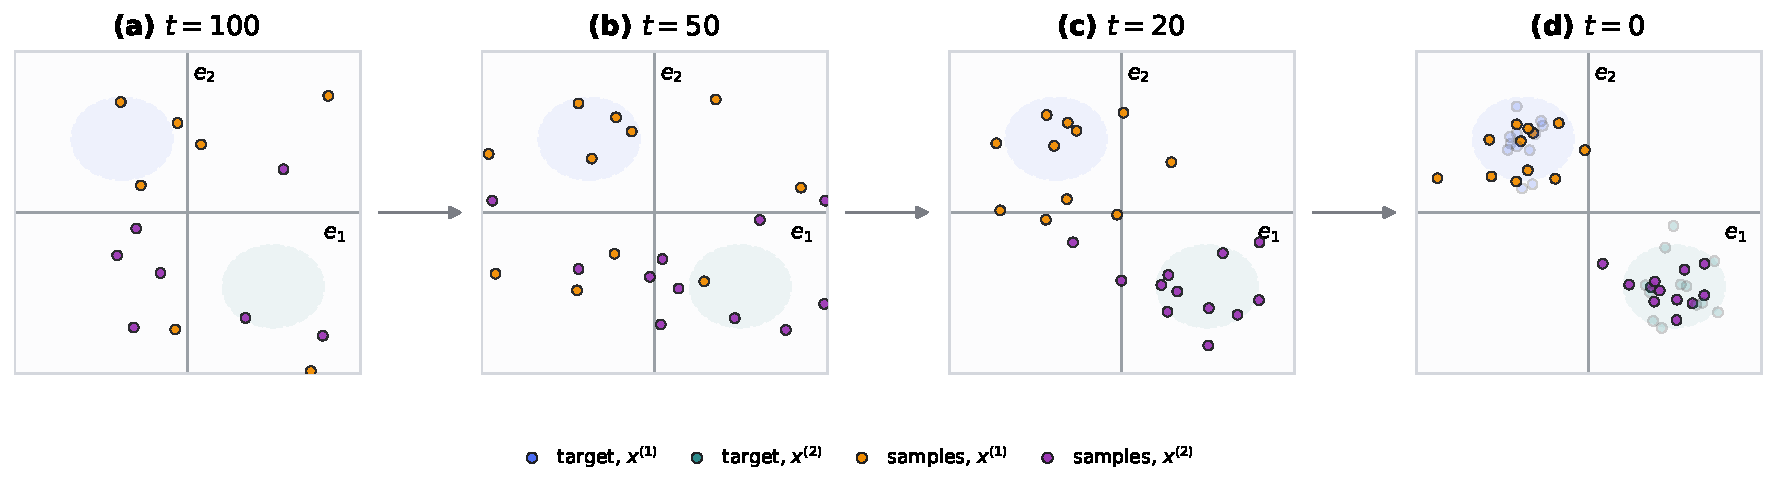
\includegraphics[width=0.98\textwidth]{figures/toy_diffusion_oracle_demo_mpl.pdf}
\caption{Oracle toy conditional diffusion trajectory on the same Gaussian conditional target. The panels show reverse-time snapshots from a 100-step diffusion process at \(t=100\), \(t=50\), \(t=20\), and \(t=0\). Starting from condition-independent noise, the reverse denoising trajectory progressively separates the conditions and contracts toward their target residual distributions. This figure is included to contrast the explicit multi-step reverse path of diffusion with the one-shot sampling path of drifting.}
\label{fig:toydiff}
\end{figure*}

\section{Experimental Setup}
\subsection{Channel models}
We benchmark four channel families.

\textbf{AWGN:}
\begin{equation}
y = x + n,
\qquad
n \sim \mathcal{N}(0,\sigma^2 I).
\end{equation}

\textbf{Rayleigh:}
the transmitted symbol is multiplied elementwise by a Rayleigh fading coefficient and then corrupted by additive Gaussian noise.

\textbf{SSPA:}
the input amplitude is passed through a smooth solid-state power amplifier nonlinearity before additive noise is applied.

\textbf{OptFib:}
we include a simplified memoryless optical-fiber proxy channel adapted from \texttt{DM\_OptFib}.
The I/Q pair is propagated through \(K_{\text{step}}\) repeated nonlinear phase rotations with per-step Gaussian noise injection.
In the current benchmark, the default parameters are \(L=5000\), \(\gamma=1.27\), \(K_{\text{step}}=50\), and \(P_n=-21.3\) dBm.

\subsection{Training protocol}
All models are trained conditionally on \(x\) in residual space.
The local benchmark configuration used for the stored comparison figures is:
\begin{itemize}
\item residual dimension \(n=2\),
\item noise standard deviation \(0.3\),
\item training set size \(30{,}000\),
\item diffusion epochs \(20\),
\item GAN epochs \(60\),
\item batch size \(256\),
\item evaluation set size \(5{,}000\),
\item hidden width \(128\) for diffusion, drifting, and GAN baselines,
\item latent dimension \(16\) for drifting and GAN generators.
\end{itemize}

For diffusion, we evaluate two horizons: \(T=20\) and \(T=100\).
At each horizon, we report full DDPM sampling, full DDIM sampling, and a reduced-step DDIM trajectory as an ablation.
For readability, the fast DDIM ablation is omitted from the main bar plot, but it is retained in the tables because it is informative about quality degradation under aggressive trajectory shortening.

In addition to the local benchmark, the repository includes a dedicated publication runner, \texttt{publication\_benchmark\_t100.py}, for multi-seed GPU evaluation.
That script uses a larger configuration with dataset size \(120{,}000\), diffusion epochs \(60\), GAN epochs \(120\), batch size \(512\), evaluation size \(20{,}000\), bootstrap confidence intervals, and pairwise win tables.

\subsection{Evaluation metric and sanity checks}
The primary metric is sliced Wasserstein distance on residual vectors:
\begin{equation}
\mathrm{SWD}\!\left(\{\hat{e}_i\}, \{e_i\}\right).
\end{equation}
In the current code, SWD is estimated using \(256\) random one-dimensional projections.
Residual-space SWD was selected over histogram \(L_1\) distance because it better captures geometry in \(\mathbb{R}^2\) and behaves more consistently across different channel families.

Several sanity checks were added to support trust in the benchmark pipeline.
These include SWD identity and symmetry tests, byte-identical reruns under fixed seeds, finite-value validation of stored JSON result files, and small cross-seed ranking checks on AWGN and OptFib.
These checks do not replace the full multi-seed publication run, but they reduce the risk that the observed comparisons are artifacts of an inconsistent implementation.

\section{Results}
\subsection{Lower-budget comparison at \(T=20\)}
Table~\ref{tab:t20} shows the lower-budget benchmark.
At this shorter horizon, drifting is already highly competitive and attains the best SWD on AWGN, Rayleigh, and OptFib.
The improved GAN baseline is also reasonably strong on SSPA.
The main takeaway is that when the diffusion budget is constrained, one-shot methods become particularly attractive.

\begin{table*}[t]
\caption{Residual SWD comparison at \(T=20\) (lower is better)}
\label{tab:t20}
\centering
\scriptsize
\begin{tabular}{lccccc}
\toprule
Channel & DDPM(20) & DDIM(20) & DDIM(10) & GAN & Drifting \\
\midrule
AWGN     & 0.0317 & 0.0979 & 0.1407 & 0.0678 & \textbf{0.0150} \\
Rayleigh & 0.0597 & 0.2668 & 0.4296 & 0.1553 & \textbf{0.0219} \\
SSPA     & 0.0366 & 0.1020 & 0.1679 & 0.0267 & \textbf{0.0191} \\
OptFib   & 0.1727 & 0.2176 & 0.4101 & 0.2963 & \textbf{0.0632} \\
\bottomrule
\end{tabular}
\end{table*}

\subsection{Main comparison at \(T=100\)}
Table~\ref{tab:t100} reports the higher-fidelity comparison with \(T=100\).
This is the fairest setting for diffusion because it allows the DDPM baseline to use the longer reverse trajectory that it benefits from.
The results show a more nuanced picture than a simple ``drifting versus diffusion'' narrative.
DDPM(100) is strongest on AWGN and SSPA, which suggests that iterative refinement remains advantageous on near-Gaussian and moderately nonlinear channels.
However, drifting remains the best model on Rayleigh and OptFib in the current benchmark, indicating that the one-shot generator is not merely a speed-oriented compromise.

\begin{table*}[t]
\caption{Residual SWD comparison at \(T=100\) (lower is better)}
\label{tab:t100}
\centering
\scriptsize
\begin{tabular}{lccccc}
\toprule
Channel & DDPM(100) & DDIM(100) & DDIM(20) & GAN & Drifting \\
\midrule
AWGN     & \textbf{0.0055} & 0.0623 & 0.2848 & 0.0713 & 0.0154 \\
Rayleigh & 0.0484 & 0.1490 & 1.0641 & 0.1459 & \textbf{0.0192} \\
SSPA     & \textbf{0.0180} & 0.1018 & 0.5833 & 0.0324 & 0.0197 \\
OptFib   & 0.1662 & 0.2754 & 2.2907 & 0.2957 & \textbf{0.0808} \\
\bottomrule
\end{tabular}
\end{table*}

The DDIM results are also informative.
Full DDIM trajectories are consistently weaker than DDPM in the present implementation, and aggressive fast-DDIM sampling degrades sharply on Rayleigh and OptFib.
This is precisely why the reduced-step DDIM bars were removed from the main figure: they dominate the plot scale without changing the qualitative conclusion.

\begin{figure*}[t]
\centering
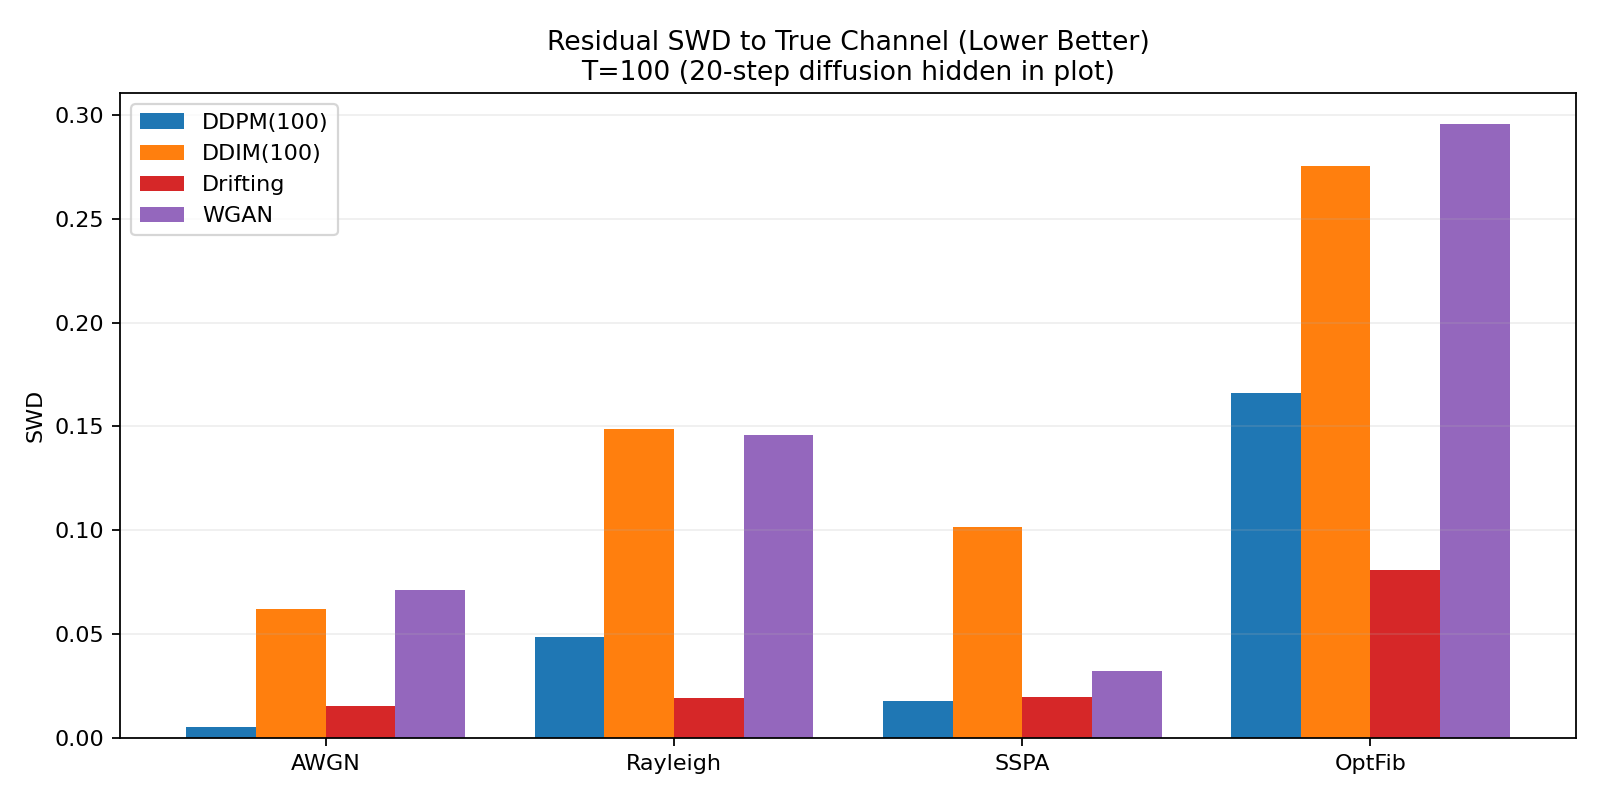
\includegraphics[width=0.9\textwidth]{figures/benchmark_channels_swd_gan_t100_ddim20_gan_fa_ge60_no20plot.png}
\caption{Residual SWD comparison across channels for the \(T=100\) benchmark. The fast reduced-step DDIM ablation is omitted for readability.}
\label{fig:bar}
\end{figure*}

\subsection{Example residual distributions}
Fig.~\ref{fig:awgn} provides a channel-level illustration on AWGN.
The residual histograms show that DDPM and DDIM capture the overall shape of the residual law, while the drifting model produces a comparably concentrated one-shot residual distribution.
The corresponding residual-SWD summary makes the ranking easier to read than a scatter plot alone.
More importantly, this figure demonstrates why a geometry-aware metric is useful: the visual overlap between methods can be deceptively similar even when the transport-based discrepancy differs.

\begin{figure}[t]
\centering
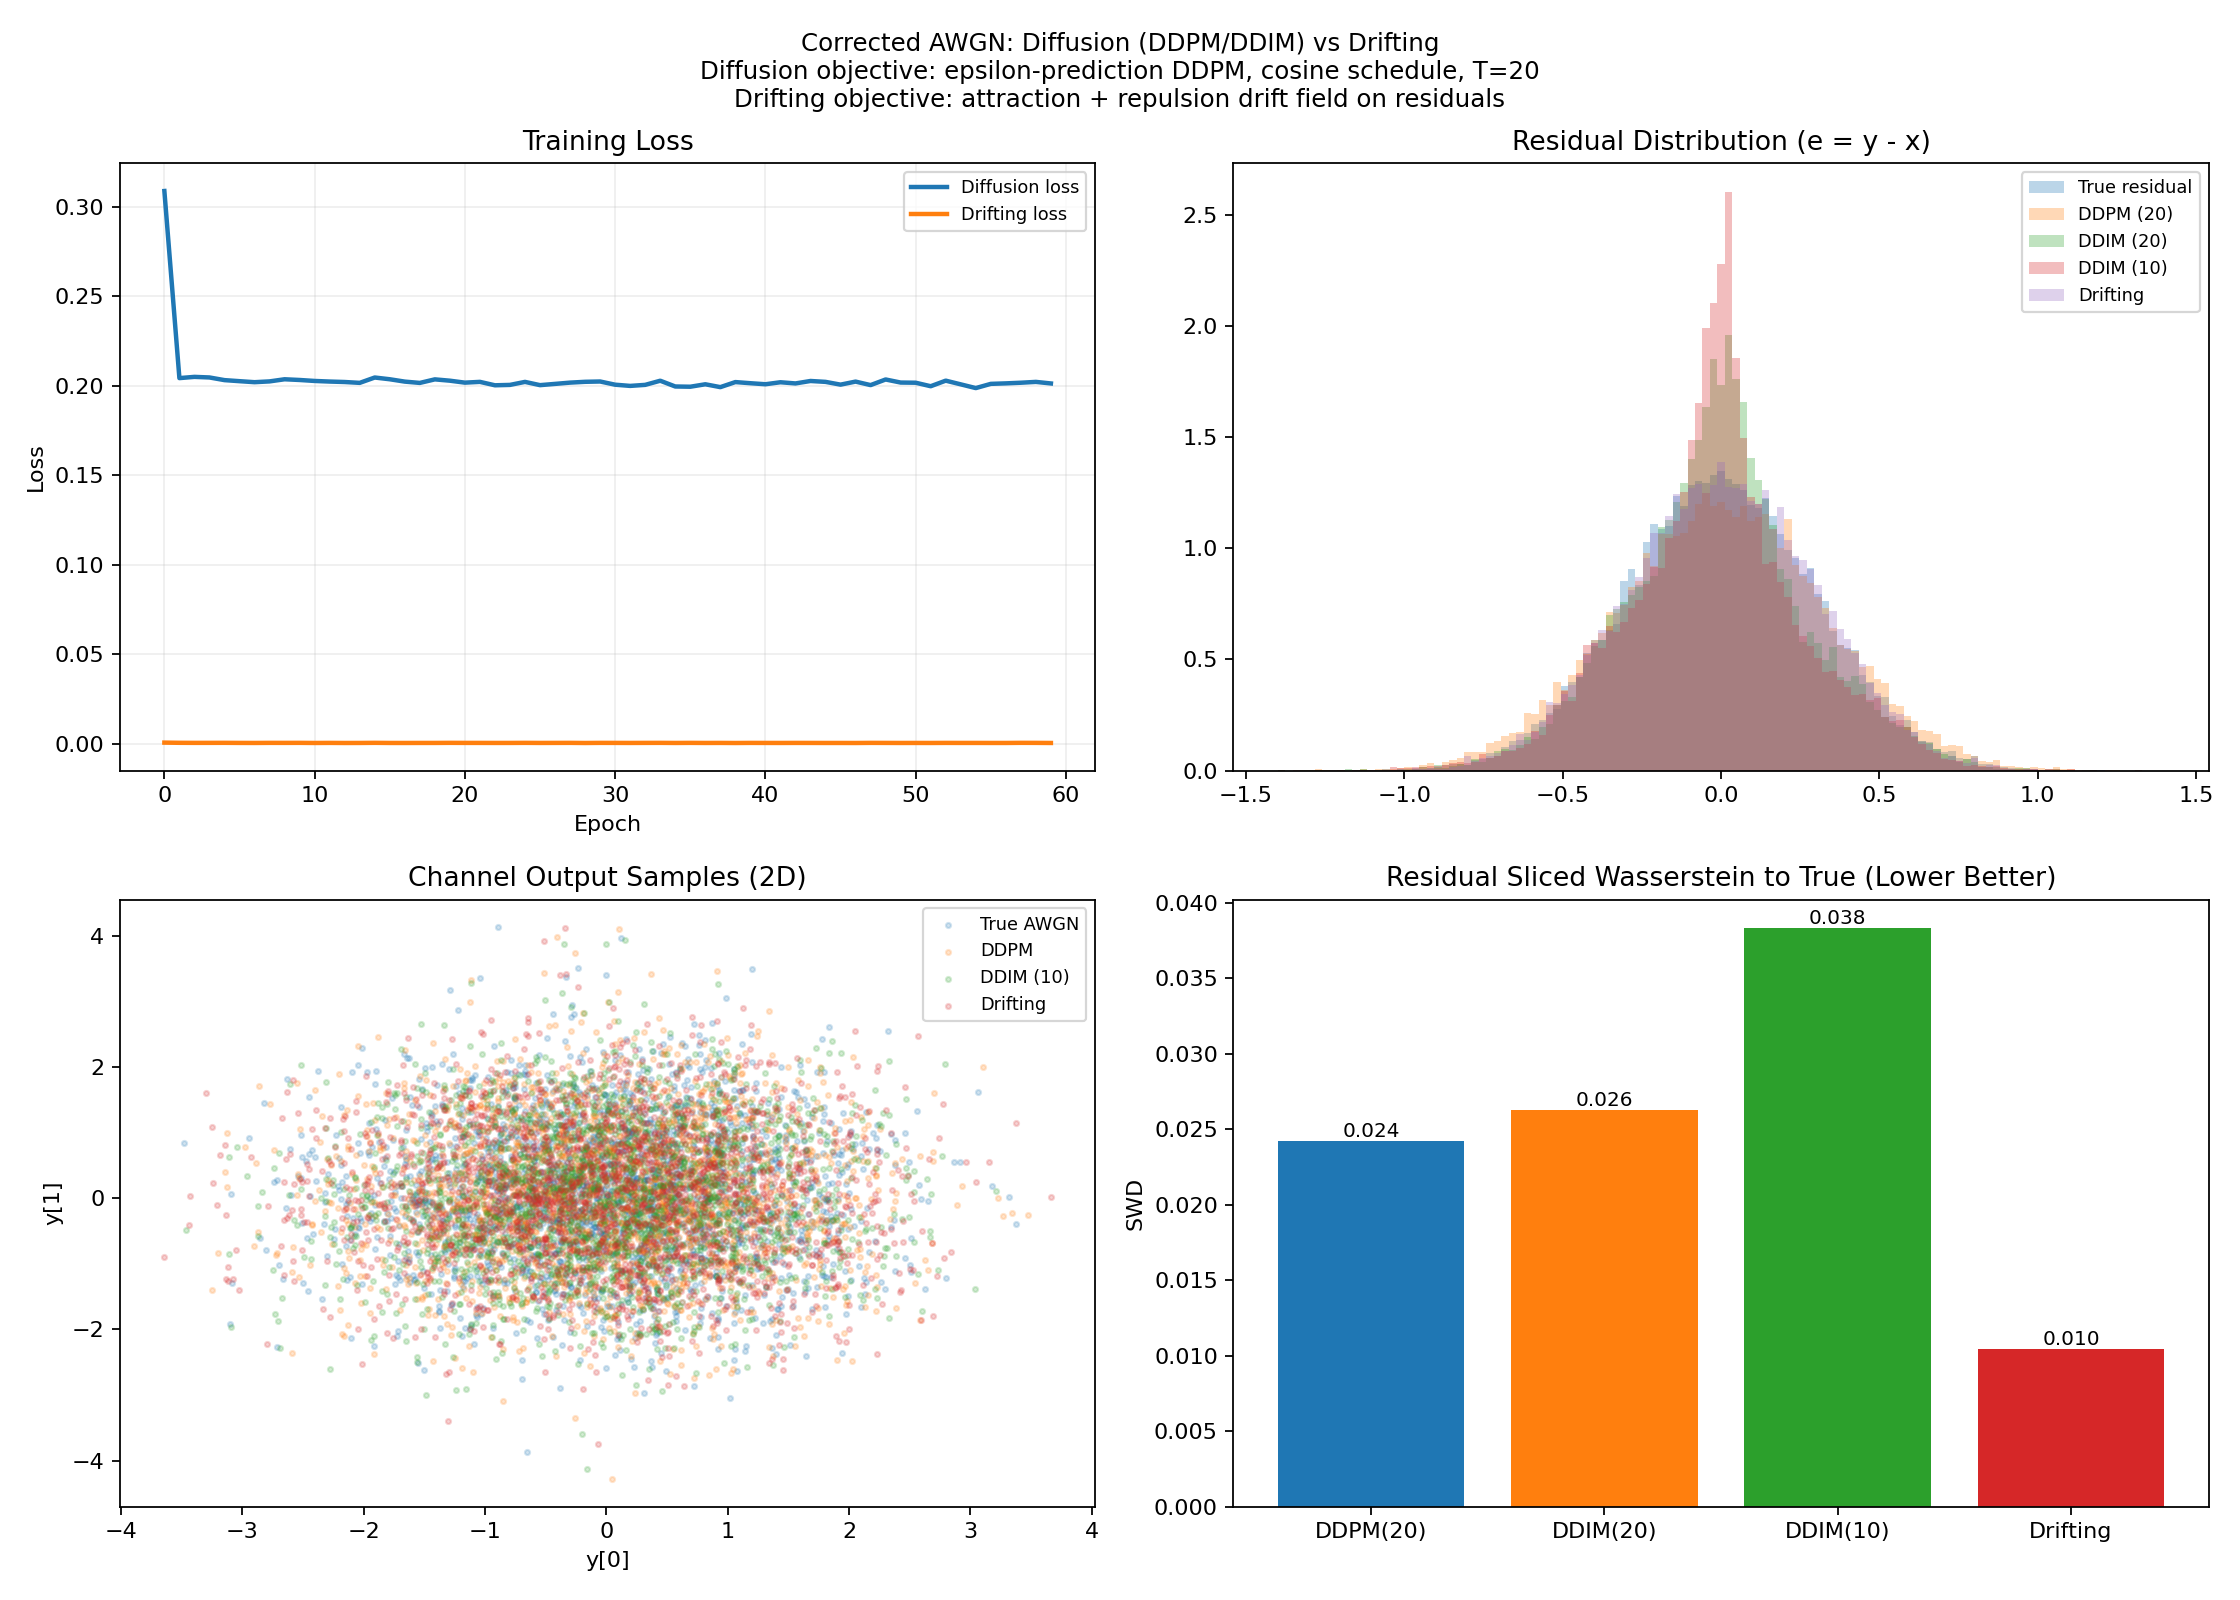
\includegraphics[width=\columnwidth]{figures/awgn_ddpm_ddim_drifting_corrected.png}
\caption{AWGN example with training curves, residual distributions, sample clouds, and residual SWD comparison.}
\label{fig:awgn}
\end{figure}

\subsection{Inference-time comparison}
The central practical motivation for drifting is inference cost.
To isolate latency from fidelity, we timed DDPM(100) and drifting separately on CPU over 20{,}480 generated samples per repeat, using batch size \(512\), \(40\) batches, and \(7\) repeats.
DDPM(100) required \(4.2612\) s per repeat, corresponding to \(4{,}806\) samples/s or \(0.2081\) ms per sample.
The one-shot drifting generator required \(0.0163\) s per repeat, corresponding to \(1.253\times 10^6\) samples/s or \(7.98\times 10^{-4}\) ms per sample.
This yields an observed speedup of \(260.8\times\) in favor of drifting.

The timing result is consistent with the model structures in Fig.~\ref{fig:schematic}.
Diffusion allocates substantial test-time computation to iterative denoising, whereas drifting allocates that work to parameter learning and uses constant-depth sampling once training is complete.
In workloads where the channel model is invoked repeatedly, this distinction can dominate overall runtime.

\subsection{Interpretation and limitations}
Several caveats are important.
First, the tables above are current single-seed benchmark results.
They are useful for method development and paper drafting, but the final publication version should be based on the multi-seed \(T=100\) runner included in the repository.
Second, the present study focuses on generator-level distributional fidelity and timing rather than on full end-to-end communication metrics such as SER or \(E_b/N_0\) curves.
Relative to \cite{paper2309}, the present draft should therefore be interpreted as a complementary benchmark on channel-distribution learning rather than as a replacement for downstream system evaluation.

Third, the drifting implementation here is deliberately pragmatic.
It is inspired by \cite{drifting} and captures the core one-shot training idea through an attraction--repulsion drift field, but it is not a claim that every modeling choice from the drifting paper has been reproduced exactly.
That said, the current results are already strong enough to justify a more systematic follow-up study.

\section{Conclusion}
This paper presented a detailed experimental draft for conditional drifting models in learned channel simulation and compared them against conditional diffusion and GAN baselines on AWGN, Rayleigh, SSPA, and optical-fiber proxy channels.
The results show a clear tradeoff.
At lower diffusion budgets, drifting is highly competitive and often strongest.
At \(T=100\), DDPM remains the best fidelity baseline on AWGN and SSPA, while drifting is strongest on Rayleigh and OptFib and preserves a one-shot inference path.
Most importantly, drifting provides a \(260.8\times\) CPU speedup over DDPM(100) in the current implementation.

These observations suggest that drifting is not only an interesting new generative-model idea, but also a practically relevant direction for communication-system channel learning.
The next steps are straightforward: run the full multi-seed publication benchmark, report confidence intervals, and extend the comparison to downstream communication metrics and more realistic optical or memory channels.

\bibliographystyle{IEEEtran}
\bibliography{references}

\end{document}
